\documentclass[leqno]{article}
\usepackage[utf8]{inputenc}
\usepackage[T1]{fontenc}
\usepackage{amsfonts}
\usepackage{fourier}
\usepackage{heuristica}
\usepackage{enumerate}
\author{Colin Roberts}
\title{MATH 570, Homework 4}
\usepackage[left=3cm,right=3cm,top=3cm,bottom=3cm]{geometry}
\usepackage{amsmath}
\usepackage[thmmarks, amsmath, thref]{ntheorem}
%\usepackage{kbordermatrix}
\usepackage{mathtools}
\usepackage{tikz-cd}

\theoremstyle{nonumberplain}
\theoremheaderfont{\itshape}
\theorembodyfont{\upshape:}
\theoremseparator{.}
\theoremsymbol{\ensuremath{\square}}
\newtheorem{proof}{Proof}
\theoremsymbol{\ensuremath{\square}}
\newtheorem{lemma}{Lemma}
\theoremsymbol{\ensuremath{\blacksquare}}
\newtheorem{solution}{Solution}
\theoremseparator{. ---}
\theoremsymbol{\mbox{\texttt{;o)}}}
\newtheorem{varsol}{Solution (variant)}

\newcommand{\tr}{\mathrm{tr}}
\newcommand{\Int}{\ensuremath{\mathrm{Int}}}
\newcommand{\N}{\ensuremath{\mathbb{N}}}
\newcommand{\Q}{\ensuremath{\mathbb{Q}}}
\newcommand{\R}{\ensuremath{\mathbb{R}}}
\newcommand{\Z}{\ensuremath{\mathbb{Z}}}
\newcommand{\cB}{\ensuremath{\mathcal{B}}}
\newcommand{\cF}{\ensuremath{\mathcal{F}}}


\begin{document}
\maketitle
\begin{large}
\begin{center}
Solutions
\end{center}
\end{large}
\pagebreak

%%%%%%%%%%%%%%%%%%%%%%%%%%%%%%%%%%%%%%%%%%%%%%%%%%%%%%%%%%%%%%%%%%%%%%%%%%%%%%%%%%%%%%%%%%%%%%%%%%%%%%%%%%%%%%%%%%%%%
%%%%%%%%%%%%%%%%%%%%%%%%%PROBLEM 1%%%%%%%%%%%%%%%%%%%%%%%%%%%%%%%%%%%%%%%%%%%%%%%%%%%%%%%%%%%%%%%%%%%%%%%%%%%%%%%%%%%%%%%%%%%%%%%%%%%%%%%%%%%%%%%%%%%%%%%%%%%%%%%%%%%%%%%%%%%%%%%%%%%%%%%%%%%%%%%%%%%%%%%%%%%%%%%%%%%%%%%%%%%%%%%%%%%%%%%%

\noindent\textbf{Problem 1.} Prove that if a coproduct exists in a category, then it is unique up to isomorphism. That is, prove that if $(S',(\iota_\alpha '))$ and $(S'',(\iota_\alpha ''))$ are both coproducts of the family of objects $(X_\alpha)_{\alpha\in A}$ then $S'$ and $S''$ are isomorphic. 

\noindent\rule[0.5ex]{\linewidth}{1pt}

\begin{proof} 
Let $(S',(\iota_\alpha ' ))$ and $(S'',(\iota_\alpha ''))$ be coproducts for the family of objects $(X_\alpha)_{\alpha \in A}$.  Then we are guaranteed unique morphisms $f'\colon S'\to S''$ and $f'' \colon S'' \to S'$ which satisfy $\iota_\alpha'' \circ f' = \iota_\alpha'$ and $\iota_\alpha' \circ f'' = \iota_\alpha''$.  Considering the diagram on page 214 of our text, we have that we can let $W=S'$ and $S''=S$ and then note that $f_\alpha = \iota_\alpha'$ and the diagram commutes with $f''\circ f'$ or $\textrm{Id}_{S'}$ in place of $f'$.  So then $f''\circ f'=\textrm{Id}_{S'}$.  An analogous argument shows that $f'\circ f'' = \textrm{Id}_{S''}$. And so we have that $S'$ and $S''$ are isomorphic by uniqueness of $f'$ and $f''$.
\end{proof}

\pagebreak

%%%%%%%%%%%%%%%%%%%%%%%%%%%%%%%%%%%%%%%%%%%%%%%%%%%%%%%%%%%%%%%%%%%%%%%%%%%%%%%%%%%%%%%%%%%%%%%%%%%%%%%%%%%%%%%%%%%%%
%%%%%%%%%%%%%%%%%%%%%%%%%PROBLEM 2%%%%%%%%%%%%%%%%%%%%%%%%%%%%%%%%%%%%%%%%%%%%%%%%%%%%%%%%%%%%%%%%%%%%%%%%%%%%%%%%%%%%%%%%%%%%%%%%%%%%%%%%%%%%%%%%%%%%%%%%%%%%%%%%%%%%%%%%%%%%%%%%%%%%%%%%%%%%%%%%%%%%%%%%%%%%%%%%%%%%%%%%%%%%%%%%%%%%%%%%


\noindent\textbf{Problem 2.} Let $(X_\alpha)_{\alpha \in A}$ be a family of topological spaces, and equip $\coprod_{\alpha \in A} X_\alpha$ with the disjoint union topology. Prove that $\coprod_{\alpha \in A} X_\alpha$ is the coproduct of $(X_\alpha)_{\alpha\in A}$ in the category of topological spaces as follows.
\begin{enumerate}[(a)]
\item Define the maps $\iota_\alpha \colon X_\alpha \to \coprod_{\alpha \in A} X_\alpha$. 
\item Prove that $(\coprod_{\alpha \in A} X_\alpha, (\iota_\alpha))$ satisfies the necessary universal property.
\end{enumerate}


\noindent\rule[0.5ex]{\linewidth}{1pt}

\begin{proof}[Part (a)]
We have that $\iota_\alpha \colon X_\alpha \to \coprod_{\alpha\in A} X_\alpha$ by $\iota_\alpha (X)=(X,\alpha)$.
\end{proof}

\begin{proof}[Part (b)]
Suppose that $W$ is a space with morphism $f_\alpha \colon X_\alpha \to W$ with $x\mapsto w$ and define $f\colon \coprod_{\alpha \in A} X_\alpha \to W$ by $(x,\alpha)\mapsto f_\alpha(X)$.  These satisfy the universal property.
\end{proof}


\pagebreak


%%%%%%%%%%%%%%%%%%%%%%%%%%%%%%%%%%%%%%%%%%%%%%%%%%%%%%%%%%%%%%%%%%%%%%%%%%%%%%%%%%%%%%%%%%%%%%%%%%%%%%%%%%%%%%%%%%%%%
%%%%%%%%%%%%%%%%%%%%%%%%%PROBLEM 3%%%%%%%%%%%%%%%%%%%%%%%%%%%%%%%%%%%%%%%%%%%%%%%%%%%%%%%%%%%%%%%%%%%%%%%%%%%%%%%%%%%%%%%%%%%%%%%%%%%%%%%%%%%%%%%%%%%%%%%%%%%%%%%%%%%%%%%%%%%%%%%%%%%%%%%%%%%%%%%%%%%%%%%%%%%%%%%%%%%%%%%%%%%%%%%%%%%%%%%%


\noindent\textbf{Problem 3.} Let $X=(\R\times \{0\})\cup (\R \times \{1\}) \subseteq \R^2$ (equipped with the standard topology). Define an equivalence relation on $X$ by declaring $(x,0)\sim (x,1)$ if $x\neq 0$. The quotient space $X/\sim$ is called the \emph{line with two origins}.
\begin{enumerate}[(a)]
\item Show that $X/\sim$ is not Hausdorff (and hence not a manifold).
\item Show that $X/\sim$ is locally Euclidean.
\end{enumerate}

\noindent\rule[0.5ex]{\linewidth}{1pt}

\begin{proof}[Part (a)]
Consider the points $p_1=(0,0)$ and $p_2=(0,1)$ which are distinct in the quotient space.  Then consider arbitrary neighborhoods $N_{\epsilon_1}(p_1)=((-\epsilon_1,\epsilon_1),0)$ and $N_{\epsilon_2}(p_1)=((-\epsilon_2,\epsilon_2),1)$ which are indeed open sets as their preimage in $X$ are open.  But note that no matter the choice of $\epsilon_1$ and $\epsilon_2$ we have that $N_{\epsilon_1}(p_1)\cap N_{\epsilon_2}(p_2)\neq \emptyset$ since $(x,0)\sim (x,1)$ for $x\neq 0$.
\end{proof}

\begin{proof}[Part (b)]
If $p=(x,0)\sim (x,1)$ for $x\neq 0$, then a neighborhood of $p$ is of the form $N_\epsilon (p)=((x-\epsilon,x+\epsilon),0)$ for $0<\epsilon<|x|$. Clearly this set is open as the preimage of $N_\epsilon(p)$ is open in $X$.  Thus a homeomorphism for these points $f\colon X/\sim \to \mathbb{R}$  is given by $f(x,0)=x$.  Which is clearly a homeomorphism.  We then define $f(0,0)=0$ and $f(0,1)=0$ which again are clearly homeomorphisms.  Just take $N_\epsilon(0,0)$ which in which we have $f(N_\epsilon(0,0))=N_\epsilon(0)\subseteq \mathbb{R}$.  A similar argument is used for $(0,1)$. 
\end{proof}

\pagebreak



%%%%%%%%%%%%%%%%%%%%%%%%%%%%%%%%%%%%%%%%%%%%%%%%%%%%%%%%%%%%%%%%%%%%%%%%%%%%%%%%%%%%%%%%%%%%%%%%%%%%%%%%%%%%%%%%%%%%%
%%%%%%%%%%%%%%%%%%%%%%%%%PROBLEM 4%%%%%%%%%%%%%%%%%%%%%%%%%%%%%%%%%%%%%%%%%%%%%%%%%%%%%%%%%%%%%%%%%%%%%%%%%%%%%%%%%%%%%%%%%%%%%%%%%%%%%%%%%%%%%%%%%%%%%%%%%%%%%%%%%%%%%%%%%%%%%%%%%%%%%%%%%%%%%%%%%%%%%%%%%%%%%%%%%%%%%%%%%%%%%%%%%%%%%%%%


\noindent\textbf{Problem 4.}  Let $X$ and $Y$ be topological spaces, and let $f\colon X \to Y$. Suppose that $X=\cup_{\alpha \in A} U_\alpha$, with $U_\alpha$ open in $X$ for all $\alpha$, and that $f\vert_{U_\alpha} \colon U_\alpha \to Y$ is continuous for all $\alpha$. Prove that $f\colon X \to Y$ is continuous.

\noindent\rule[0.5ex]{\linewidth}{1pt}

\begin{proof}
Consider an arbitrary open set $V\subseteq Y$.  Then we have that $(f\vert_{U_\alpha})^{-1}(V)=U_\alpha\cap f^{-1}(V)$ which is open in $X$.  So consider now $\cup_{\alpha \in A} (f\vert_{U_\alpha})^{-1}(V)=\cup_{\alpha \in A} (U_\alpha \cap f^{-1}(V)) = f^{-1}(V)\cap (\cup_{\alpha \in A}(U_\alpha))=f^{-1}(V)\cap X=f^{-1}(V)$ which is open since the arbitrary union of open sets is open.  Thus $f$ is continuous.
\end{proof}


\pagebreak

%%%%%%%%%%%%%%%%%%%%%%%%%%%%%%%%%%%%%%%%%%%%%%%%%%%%%%%%%%%%%%%%%%%%%%%%%%%%%%%%%%%%%%%%%%%%%%%%%%%%%%%%%%%%%%%%%%%%%
%%%%%%%%%%%%%%%%%%%%%%%%%PROBLEM%%%%%%%%%%%%%%%%%%%%%%%%%%%%%%%%%%%%%%%%%%%%%%%%%%%%%%%%%%%%%%%%%%%%%%%%%%%%%%%%%%%%%%%%%%%%%%%%%%%%%%%%%%%%%%%%%%%%%%%%%%%%%%%%%%%%%%%%%%%%%%%%%%%%%%%%%%%%%%%%%%%%%%%%%%%%%%%%%%%%%%%%%%%%%%%%%%%%%%%%%%


\noindent\textbf{Problem 5.}  Make a M{\"o}bius band out of a strip of paper, and then cut it along its central circle. Now, draw a picture to show that identifying diametrically opposite points on one of the boundary circles of a cylinder creates a M{\"o}bius band. That is, draw a picture to show that if you take a cylinder $S^1 \times [0,1]=\{(x,y,z)\vert x^2+y^2=1 \textrm{ and } 0\leq z\leq 1\}$ and identify each $(x,y,1)$ with $(-x,-y,1)$, then you get a M{\"o}bius band.

\noindent\rule[0.5ex]{\linewidth}{1pt}

\begin{proof}
\begin{figure}[h]
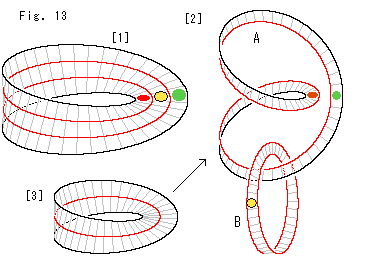
\includegraphics[scale=1]{mobius.png}
\end{figure}
In this picture we can see that we can glue the antipodal edges of the cylinder A shown in [2] (disregard the extra M{\''o}bius band cut out) and achieve the band shown in [3].  I remember doing this problem with you last year and drawing is hard, so hopefully this suffices.  Also I think it's cool you can cut the twice twisted cylinder in half again and you get two disjoint pieces which in some sense shows that it is topologically a cylinder!
\end{proof}


\pagebreak



\end{document}

